% Prof. Dr. Ausberto S. Castro Vera
% UENF - CCT - LCMAT - Curso de Ci\^{e}ncia da Computa\c{c}\~{a}o
% Campos, RJ,  2021
% Disciplina: Paradigmas de Linguagens de Programa\c{c}\~{a}o



\chapter{ Aplica\c{c}\~{o}es da Linguagem JavaScript}

O capítulo abaixo irá demonstrar implementações em JavaScript de aplicações ou estruturas de dados conhecidas. O código será explicado nos comentários e além disso, em alguns casos o código será feito em html, CSS e JavaScript. 


    \section{Pilha Implementação}
    \begin{lstlisting}
    	let stack = [];
    	
    	stack.push(1);
    	console.log(stack); // [1]
    	
    	stack.push(2);
    	console.log(stack); // [1,2]
    	
    	stack.push(3);
    	console.log(stack); // [1,2,3]
    	
    	stack.push(4);
    	console.log(stack); // [1,2,3,4]
    	
    	stack.push(5);
    	console.log(stack); // [1,2,3,4,5]
    \end{lstlisting}
    O conteúdo foi retirado de: \url{https://www.javascripttutorial.net/javascript-stack/}

	\subsection{Prints Pilha}
	
	



    \section{Árvore de Busca Binária}
    Código retirado de: \url{https://www.geeksforgeeks.org/implementation-binary-search-tree-javascript/}
    \begin{lstlisting}
    // Node class
    class Node
    {
    constructor(data)
    {
    this.data = data;
    this.left = null;
    this.right = null;
    }
    }
    
    // Binary Search tree class
    class BinarySearchTree
    {
    constructor()
    {
    // root of a binary search tree
    this.root = null;
    }
    
    // function to be implemented
    // insert(data)
    // remove(data)
    insert(data)
    {
    // Creating a node and initialising
    // with data
    var newNode = new Node(data);
    
    // root is null then node will
    // be added to the tree and made root.
    if(this.root === null)
    this.root = newNode;
    else
    
    // find the correct position in the
    // tree and add the node
    this.insertNode(this.root, newNode);
    }
    
    // Method to insert a node in a tree
    // it moves over the tree to find the location
    // to insert a node with a given data
    insertNode(node, newNode)
    {
    // if the data is less than the node
    // data move left of the tree
    if(newNode.data < node.data)
    {
    // if left is null insert node here
    if(node.left === null)
    node.left = newNode;
    else
    
    // if left is not null recur until
    // null is found
    this.insertNode(node.left, newNode);
    }
    
    // if the data is more than the node
    // data move right of the tree
    else
    {
    // if right is null insert node here
    if(node.right === null)
    node.right = newNode;
    else
    
    // if right is not null recur until
    // null is found
    this.insertNode(node.right,newNode);
    }
    }
    search(node, data)
    {
    // if trees is empty return null
    if(node === null)
    return null;
    
    // if data is less than node's data
    // move left
    else if(data < node.data)
    return this.search(node.left, data);
    
    // if data is less than node's data
    // move left
    else if(data > node.data)
    return this.search(node.right, data);
    
    // if data is equal to the node data
    // return node
    else
    return node;
    }
    
    // returns root of the tree
    getRootNode()
    {
    return this.root;
    }
    // finds the minimum node in tree
    // searching starts from given node
    findMinNode(node)
    {
    // if left of a node is null
    // then it must be minimum node
    if(node.left === null)
    return node;
    else
    return this.findMinNode(node.left);
    }
    // Performs postorder traversal of a tree
    postorder(node)
    {
    if(node !== null)
    {
    this.postorder(node.left);
    this.postorder(node.right);
    console.log(node.data);
    }
    }
    // Performs preorder traversal of a tree
    preorder(node)
    {
    if(node !== null)
    {
    console.log(node.data);
    this.preorder(node.left);
    this.preorder(node.right);
    }
    }
    
    // helper method that calls the
    // removeNode with a given data
    remove(data)
    {
    // root is re-initialized with
    // root of a modified tree.
    this.root = this.removeNode(this.root, data);
    }
    
    // Method to remove node with a
    // given data
    // it recur over the tree to find the
    // data and removes it
    removeNode(node, key)
    {
    
    // if the root is null then tree is
    // empty
    if(node === null)
    return null;
    
    // if data to be delete is less than
    // roots data then move to left subtree
    else if(key < node.data)
    {
    node.left = this.removeNode(node.left, key);
    return node;
    }
    
    // if data to be delete is greater than
    // roots data then move to right subtree
    else if(key > node.data)
    {
    node.right = this.removeNode(node.right, key);
    return node;
    }
    
    // if data is similar to the root's data
    // then delete this node
    else
    {
    // deleting node with no children
    if(node.left === null && node.right === null)
    {
    node = null;
    return node;
    }
    
    // deleting node with one children
    if(node.left === null)
    {
    node = node.right;
    return node;
    }
    
    else if(node.right === null)
    {
    node = node.left;
    return node;
    }
    
    // Deleting node with two children
    // minimum node of the right subtree
    // is stored in aux
    var aux = this.findMinNode(node.right);
    node.data = aux.data;
    
    node.right = this.removeNode(node.right, aux.data);
    return node;
    }
    
    // search for a node with given data
    
    }
    // Performs inorder traversal of a tree
    inorder(node)
    {
    if(node !== null)
    {
    this.inorder(node.left);
    console.log(node.data);
    this.inorder(node.right);
    }
    }
    
    
    // Helper function
    // findMinNode()
    // getRootNode()
    // inorder(node)
    // preorder(node)			
    // postorder(node)
    // search(node, data)
    }
    
    // create an object for the BinarySearchTree
    var BST = new BinarySearchTree();
    
    // Inserting nodes to the BinarySearchTree
    BST.insert(15);
    BST.insert(25);
    BST.insert(10);
    BST.insert(7);
    BST.insert(22);
    BST.insert(17);
    BST.insert(13);
    BST.insert(5);
    BST.insert(9);
    BST.insert(27);
    
    //		 15
    //		 / \
    //	 10 25
    //	 / \ / \
    //	 7 13 22 27
    //	 / \ /
    // 5 9 17
    
    var root = BST.getRootNode();
    
    // prints 5 7 9 10 13 15 17 22 25 27
    BST.inorder(root);
    
    // Removing node with no children
    BST.remove(5);
    
    
    //		 15
    //		 / \
    //	 10 25
    //	 / \ / \
    //	 7 13 22 27
    //	 \ /
    //	 9 17
    
    
    var root = BST.getRootNode();
    
    // prints 7 9 10 13 15 17 22 25 27
    BST.inorder(root);
    
    // Removing node with one child
    BST.remove(7);
    
    //		 15
    //		 / \
    //	 10 25
    //	 / \ / \
    //	 9 13 22 27
    //		 /
    //		 17
    
    
    var root = BST.getRootNode();
    
    // prints 9 10 13 15 17 22 25 27
    BST.inorder(root);
    
    // Removing node with two children
    BST.remove(15);
    
    //		 17
    //		 / \
    //	 10 25
    //	 / \ / \
    //	 9 13 22 27
    
    var root = BST.getRootNode();
    console.log("inorder traversal");
    
    // prints 9 10 13 17 22 25 27
    BST.inorder(root);
    
    console.log("postorder traversal");
    BST.postorder(root);
    console.log("preorder traversal");
    BST.preorder(root);
    
    \end{lstlisting}
    
    \subsection{BST Prints}
    Abaixo se encontram imagens do código e do resultado, respectivamente.
    \begin{figure}[H]
    
    	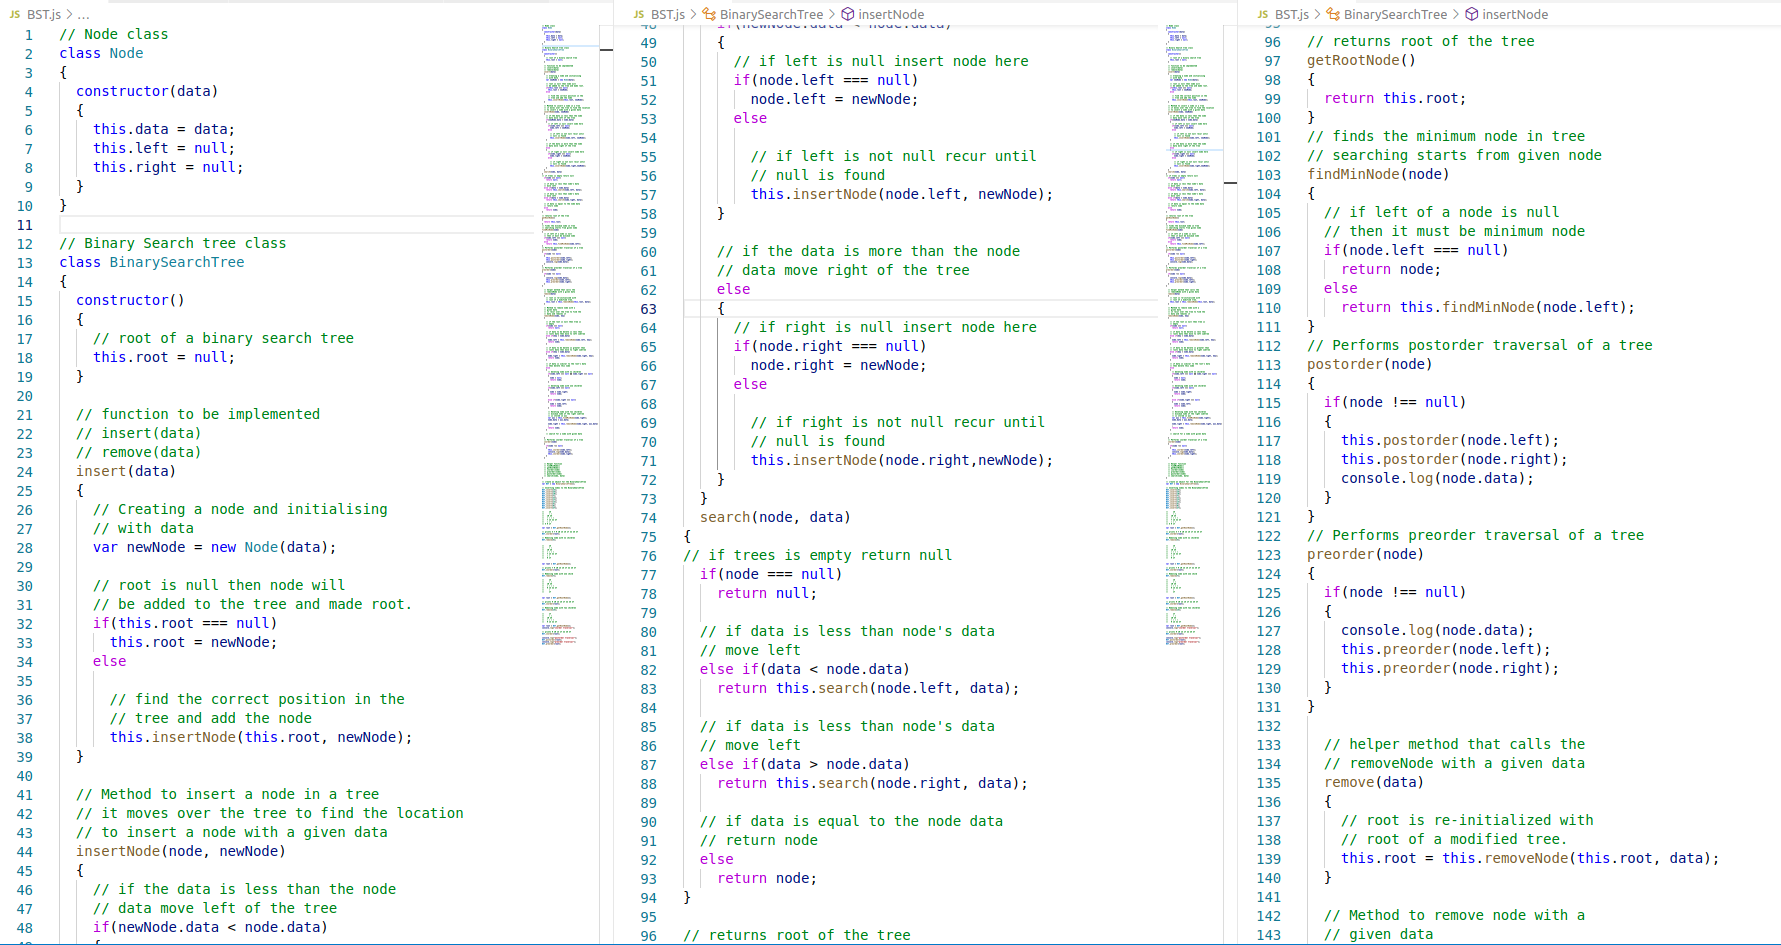
\includegraphics[width=1.1\linewidth]{Pictures/BST_Code1}
    	\caption{}
    	\label{fig:bstcode1}
    \end{figure}
    \begin{figure}[H]
    	\centering
    	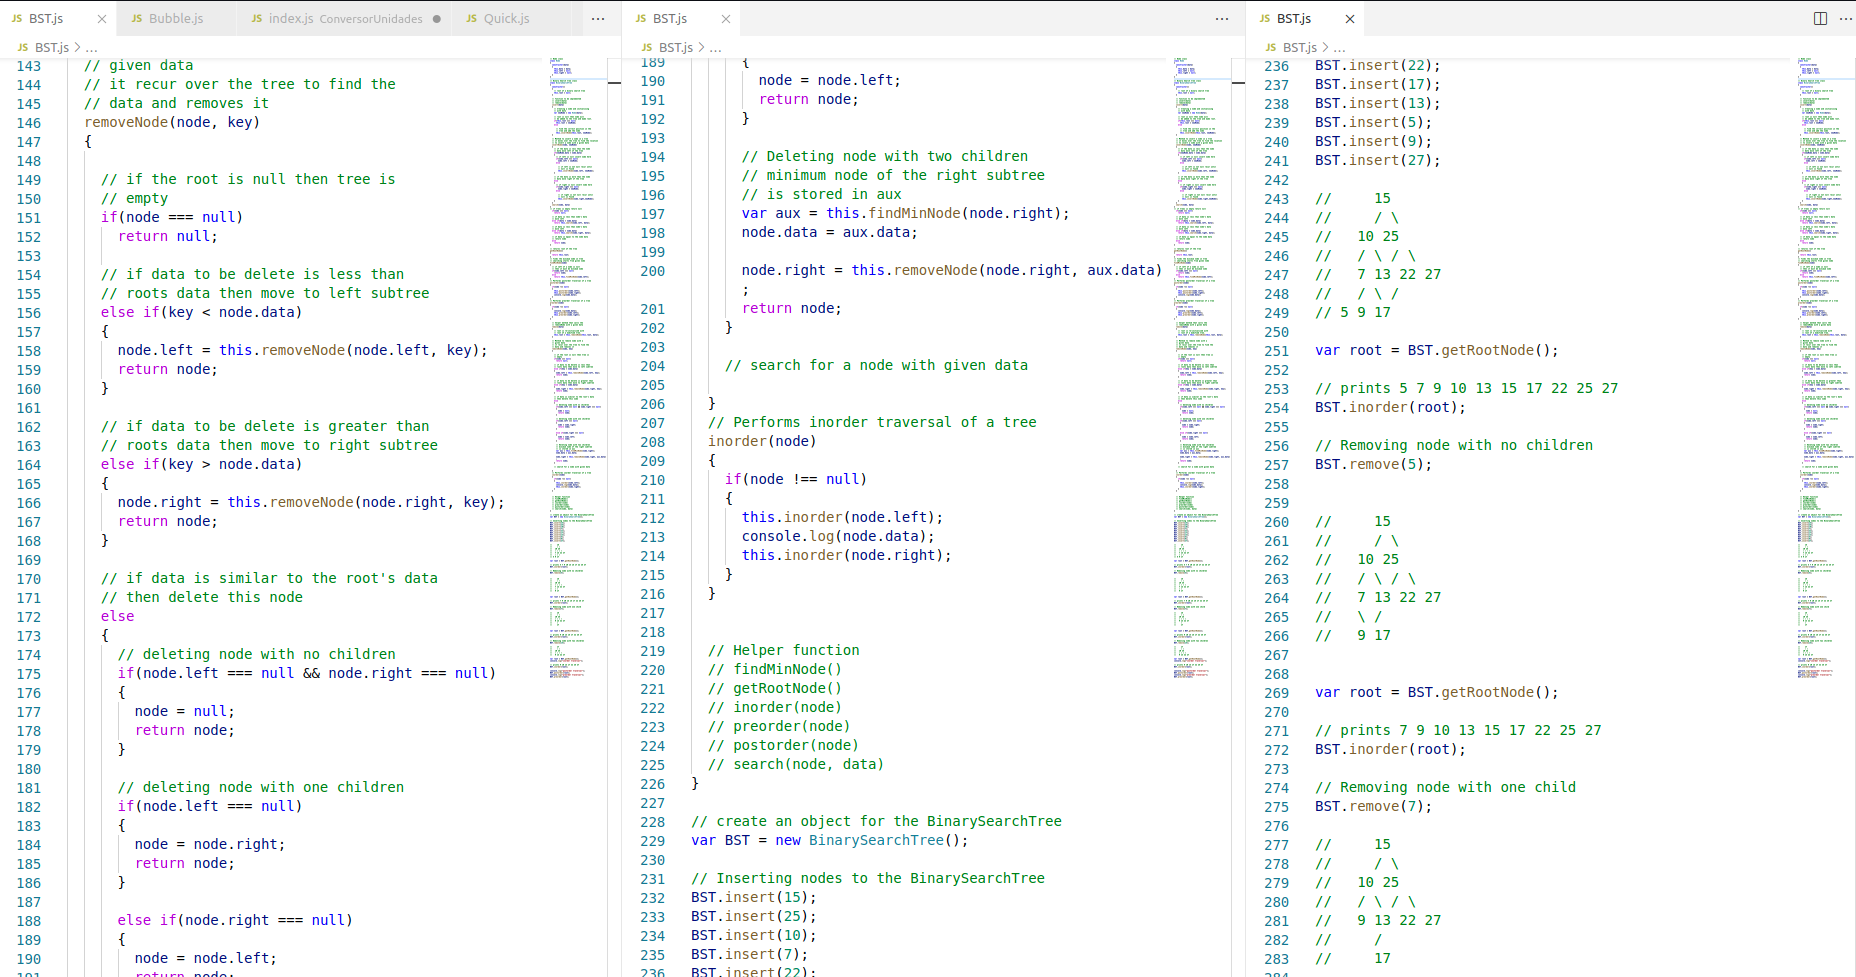
\includegraphics[width=1.1\linewidth]{Pictures/BST_Code2}
    	\caption{}
    	\label{fig:bstcode2}
    \end{figure}
    \begin{figure}[H]
    	\centering
    	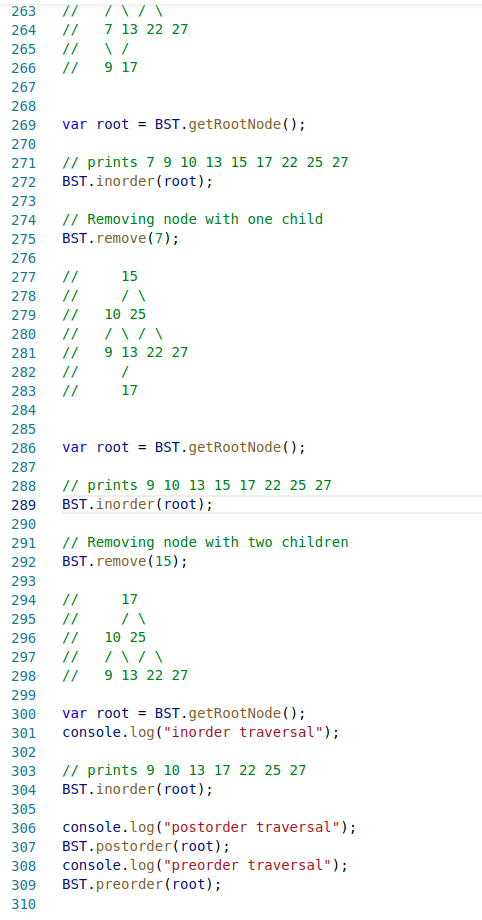
\includegraphics[width=0.9\linewidth]{Pictures/BST_Code3}
    	\caption{}
    	\label{fig:bstcode3}
    \end{figure}
    \begin{figure}[H]
    	\centering
    	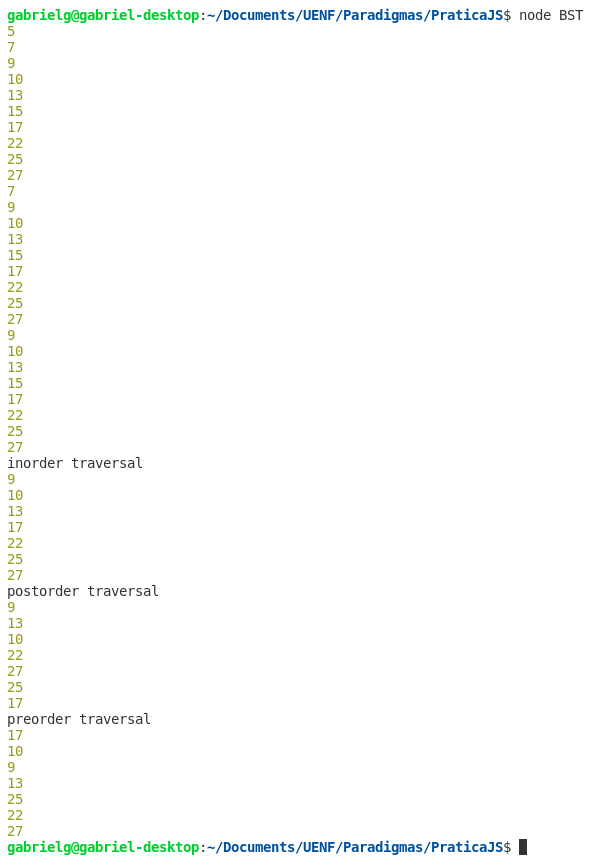
\includegraphics[width=0.9\linewidth]{Pictures/BST_Result}
    	\caption{}
    	\label{fig:bstresult}
    \end{figure}
    


    \section{Calculadora}
    O exemplo abaixo foi feito em JavaScript com HTML e CSS e interpretado pelo navegador.
    \begin{lstlisting}
    var valor1, valor2, operador;
    var readlineSync = require('readline-sync');
    operador = readlineSync.question("Qual operacao deseja efetuar (+) (-) (*) (/)? : \n");
    valor1 = parseFloat(readlineSync.question("Insira o primeiro numero: \n"));
    valor2 = parseFloat(readlineSync.question("Insira o segundo numero: \n"));
    
    function calcular(operator, value1, value2) {
    if (operator == "+") {
    return value1 + value2;
    } else if
    (operator == "-") {
    return value1 - value2;
    } else if
    (operator == "*") {
    return value1 * value2;
    } else if
    (operator == "/") {
    return value1 / value2;
    } else {
    throw new Error('Operacao invalida');
    }
    }
    
    
    console.log('O resultado e: ', calcular(operador, valor1, valor2))     
    \end{lstlisting}
    
    \subsection{Prints Calculadora}
	
	Imagens do código e do resultado, respectivamente: 
	\begin{figure}[H]
		\centering
		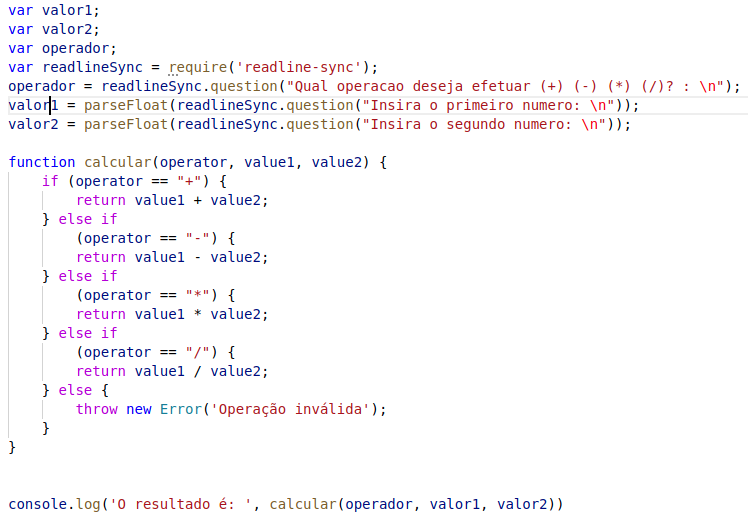
\includegraphics[width=0.9\linewidth]{Pictures/CalcCode}
		\caption{}
		\label{fig:calccode}
	\end{figure}
	\begin{figure}[H]
		\centering
		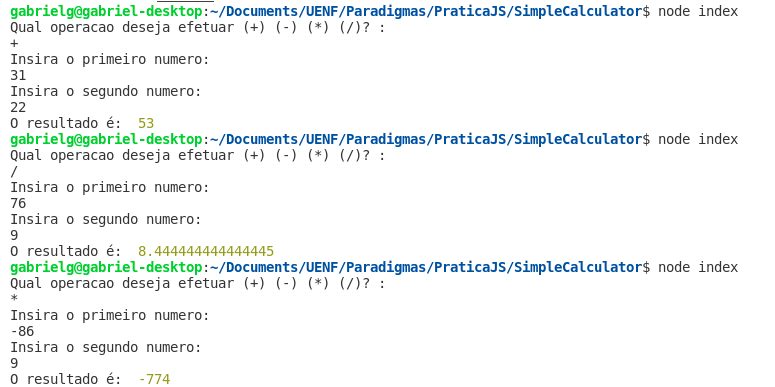
\includegraphics[width=0.9\linewidth]{Pictures/CalcResult}
		\caption{}
		\label{fig:calcresult}
	\end{figure}
	



    \section{Implementação do QuickSort}
	O algoritmo QuickSort é feito da seguinte forma no JavaScript:
	\newline
\begin{lstlisting}

// basic implementation, where pivot is the first element
function quickSortBasic(array) {
if(array.length < 2) {
return array;
}

var pivot = array[0];
var lesserArray = [];
var greaterArray = [];

for (var i = 1; i < array.length; i++) {
if ( array[i] > pivot ) {
greaterArray.push(array[i]);
} else {
lesserArray.push(array[i]);
}
}

return quickSortBasic(lesserArray).concat(pivot, quickSortBasic(greaterArray));
}

/******************* Testing Quick sort algorithm *********************/

// Returns a random integer between min (inclusive) and max (inclusive). Using Math.round() will give a non-uniform distribution, which we dont want in this case.

function getRandomInt(min, max) {
return Math.floor(Math.random() * (max - min + 1)) + min;
// By adding 1, I am making the maximum inclusive ( the minimum is inclusive anyway). Because, the Math.random() function returns a floating-point, pseudo-random number in the range from 0 inclusive up to but not including 1
}

var arr = [];

for (var i = 0; i < 10; i++) { //initialize a random integer unsorted array
arr.push(getRandomInt(1, 100));
}

console.log("Unsorted array: ");
console.log(arr); //printing unsorted array

arr = quickSortBasic(arr, 0, arr.length - 1);
console.log("Sorted array: ");
console.log(arr);


\end{lstlisting}
O código foi retirado de:
\url{https://javascript.plainenglish.io/quick-sort-algorithm-in-javascript-5cf5ab7d251b}


\subsection{Prints QuickSort}
	Código Fonte e imagem do resultado, respectivamente:
	\begin{figure}[H]
		\centering
		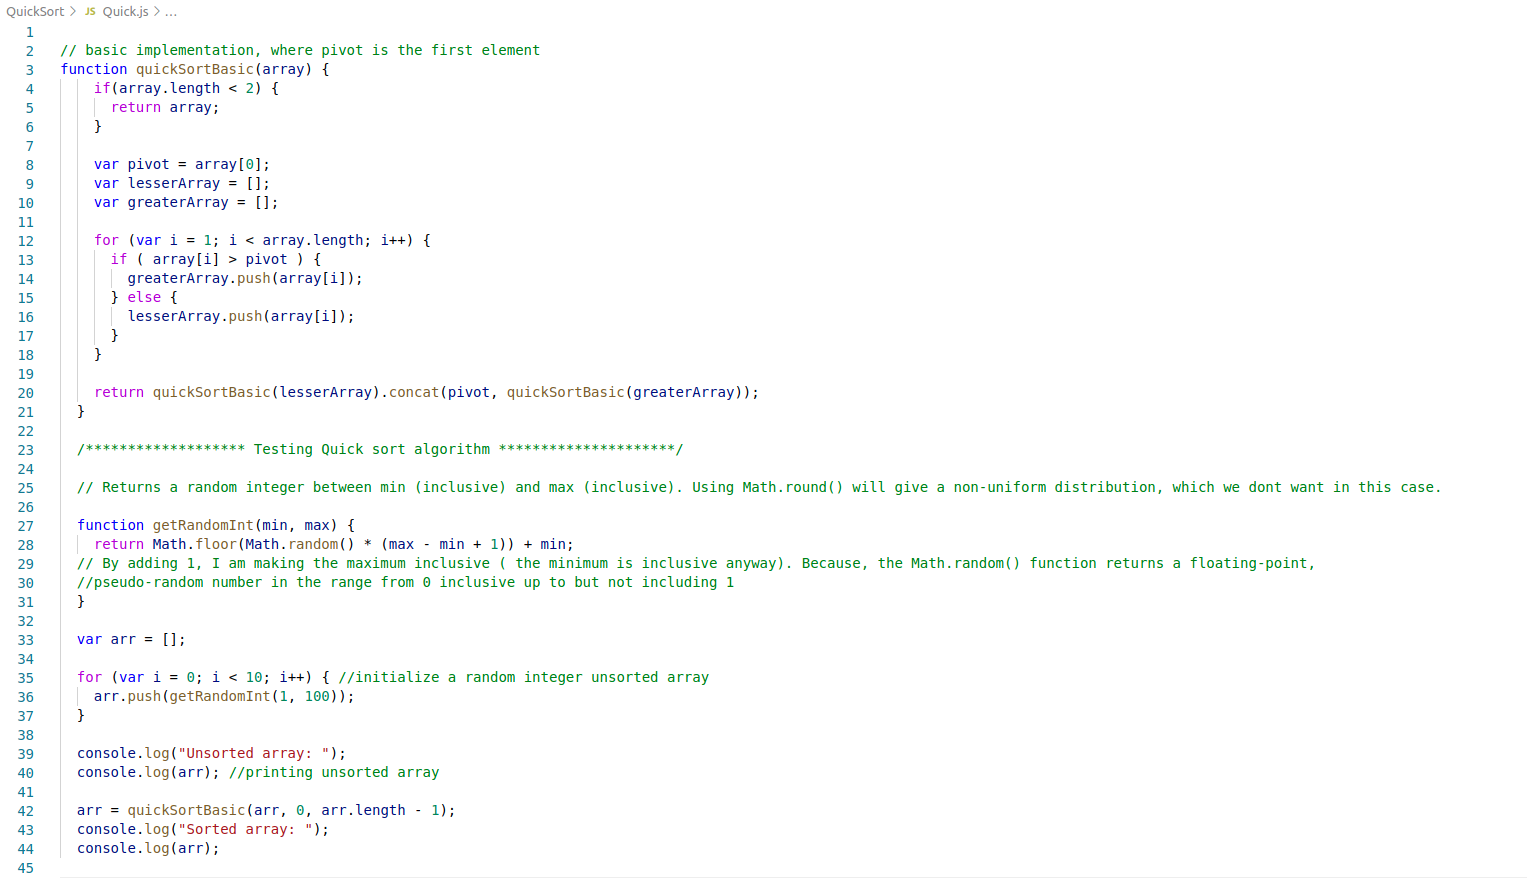
\includegraphics[width=0.95\linewidth]{Pictures/QuickCode}
		\caption{}
		\label{fig:quickcode}
	\end{figure}
	
	\begin{figure}[H]
		\centering
		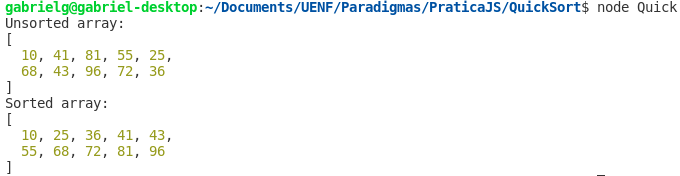
\includegraphics[width=0.95\linewidth]{Pictures/QuickResult}
		\caption{}
		\label{fig:quickresult}
	\end{figure}
	
	
	
 \section{Conversor de Temperatura}
 O código abaixo foi feito utilizando o módulo 'prompt-sync'.
 \begin{lstlisting}
 // TC/5 = (TF-32)/9 = (TK-273)/5
 
 const prompt = require('prompt-sync')();
 
 const temperatura = Number(prompt('Qual temperatura? '));
 
 
 const escala = prompt('Qual a escala da temperatura inserida? (1: Celsius; 2: Fahrenheit; 3: Kelvin)');
 
 switch(escala) {
 case '1':
 temperatura_fahrenheit = (temperatura/5)*9+32;
 temperatura_kelvin = (temperatura + 273.15);
 console.log("A temperatura: ", temperatura_kelvin, "K e ", temperatura_fahrenheit, "graus F");
 break;
 case '2':
 temperatura_celsius = ((temperatura-32)/9)*5;
 temperatura_kelvin = ((temperatura-32)/9)*5+273.15;
 console.log("A temperatura: ", temperatura_celsius, "graus C e ", temperatura_kelvin, "K");
 break;
 
 case '3':
 temperatura_fahrenheit = ((temperatura-273.15)/5)*9+32;
 temperatura_celsius = (temperatura)-273.15;
 console.log("A temperatura: ", temperatura_fahrenheit, "graus F e ", temperatura_celsius, "graus C")
 break;
 
 default:
 console.log('Insira uma escala valida de 1 a 3.');
 }
 \end{lstlisting}
 
 \subsection{Conversor de Temperatura Imagens}
 Código fonte e imagem do resultado:
\begin{figure}[h]
	\centering
	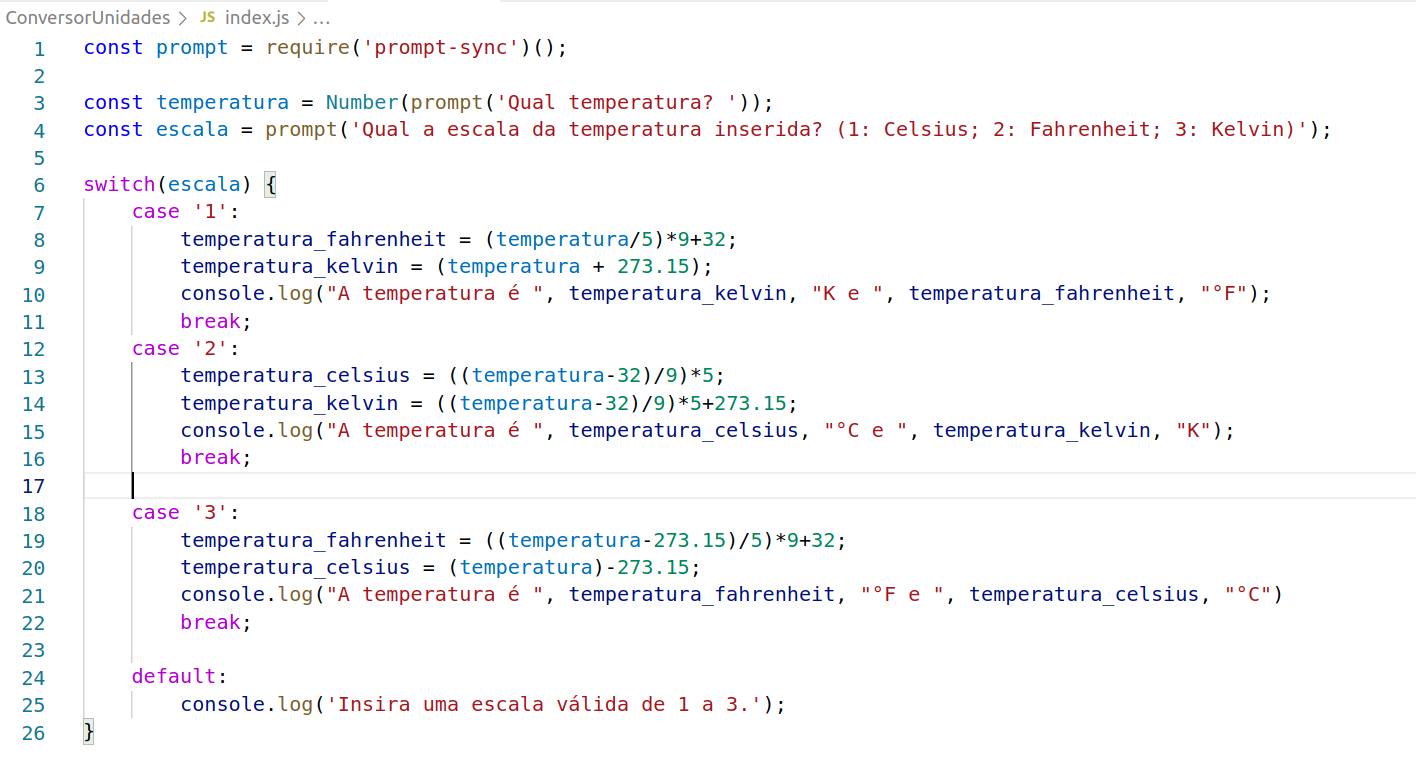
\includegraphics[width=1\linewidth]{Pictures/ConversorTempCode}
	\caption{}
	\label{fig:conversortempcode}
\end{figure}
\begin{figure}[h]
	\centering
	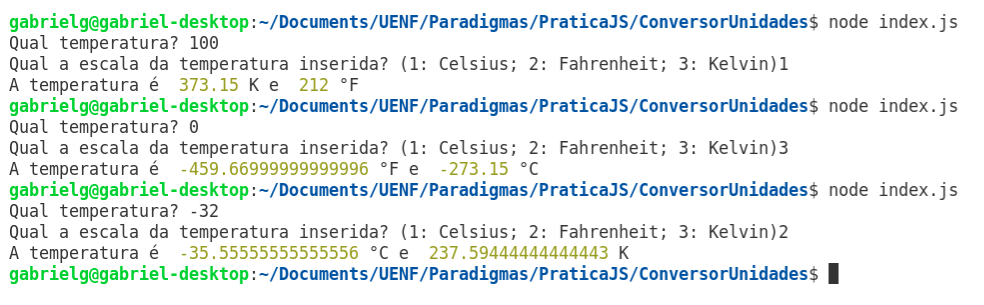
\includegraphics[width=0.9\linewidth]{Pictures/ConversorTempResultado}
	\caption{}
	\label{fig:conversortempresultado}
\end{figure}

	
	
	


	